\documentclass{article}
\usepackage[pdftex]{color}
\usepackage{graphicx}
\begin{document}

\def\path#1{#1}

\long\def\issue#1{{\color{red} #1}}

\section{Building Cardioid}

Cardioid has been designed to be portable to a wide variety of systems.
If you are building on a system that is recognized by the build system
you should only have to enter the src directory and type make.  The next
few paragraphs describe the proceedure to follow if your build host is
not recognized.

Cardioid's build system uses a hostname based configuration system
rather than an architecture based configuration (i.e., uname or
similar).  Over the years we have found that using hostnames allows us
to easily work around subtle hardware or environmental difference that
are hard to detect otherwise.  We also find that the number of build
hosts is relatively small so this system is easy to maintain, especially
compared to the complexity of a tool like autoconf.

To configure the build system for a new host, edit
\path{src/Makefile.arch} and add a conditional block for your build
host.  Note that we trim trailing digits from the host name to account
for the fact that many clusters have several front-end nodes with names
that differ only by trailing digits.  If your host is sufficiently
similar to one that is already configured you may be able to use one of
the existing values for ARCHGUESS.  If not, you will need to specify a
new value and create the corresponding \path{.mk} file with the
characteristics of your build host.  Use one of the existing files as a
guide.

\subsection{Build Targets}

The default cardioid build target is an optimized binary.  This binary
will be placed in \path{../bin} relative to the \path{src} directory.

Several other build targets exist:
\par\noindent
\begin{description}
\item[debug]  Builds a binary with debugging information.  Optimizations are
  disabled to make debugging easier.
\item[profile] Builds a binary that will generate profiling information
  suitable for use with gprof.
\item[clean]  Deletes many of the files generated by the build include
  object files and binaries.
\item[distclean] Deletes all files generated by the build.
\item[ddcMD\_dist] Useful for ddcMD developers.  See
  subsection~\ref{ssec:ddcMD}.
\end{description}

\subsection{Relationship to ddcMD}
\label{ssec:ddcMD}

Cardioid uses a number of sorce code files that are developed and
maintained as part of ddcMD.  For various reasons, these files have
never been organized into a separately maintained library.  This makes
it a challenge to use these files in the Cardioid build.  If you are not
a ddcMD developer, the build system takes care of just about everything.
The only things you need to know about ddcMD are:
\begin{enumerate}
\item The files in the \path{src/ddcMD\_files} subdirectory are generated
  files and you should not change them.  
\item You should not put files in \path{src/ddcMD\_files} since this
  directory is deleted by the distclean target of make.
\item The files that Cardioid needs from ddcMD are distributed as a
  compressed tarfile as part of the source code distribution.
  Occaisionally this distribution needs updating.  When this happens you
  will need to make distclean to erase stale files.  Whenever you see
  build errors after an svn update your first reaction should always be
  to make distclean.
\end{enumerate}

If you are a ddcMD developer, especially if you make changes to the
files that are used by Cardioid, you should understand how Cardioid
interacts with ddcMD, how to safely make changes to ddcMD files, and how
to update the tar file in the Carioid distributon that contains ddcMD
files.

All of the ddcMD files used by Cardioid are listed in the DDCMD\_FILES
variable in the Cardioid Makefile.  The Cardioid build system creates
symbolic links to all of these files and then processes them as if they
were regular source files in the \path{src} directory.  The script
\path{mkLinks\_ddcMD.sh} is responsible for creating the symbolic links.
It is automatically invoked by make when necessary.  
Developers of ddcMD should keep a ddcMD source tree in one of the
locations listed in the search path in \path{mkLinks\_ddcMD.sh}.  This
will ensure that the symbolic links in the Cardioid source tree are
pointing at active ddcMD sources that are under version control.

If it is necessary to modify the ddcMD sources that are used by
Cardioid, the changes should be made in the linked ddcMD source tree.
Once a developer is satisfied the changes are correct the following
procedure is used to create the new tarfile that other Cardioid
developers and users will need.  Don't skip steps.
\begin{enumerate}
\item Confirm that both Cardioid and ddcMD build and function correctly
  with the changes.
\item Use svn to commit the changed ddcMD code to the ddcMD repository.
\item Update your ddcMD sources.  
\item Ensure that the svnversion command returns a single number without
  a trailing ``M'' or a pair of numbers separated by a ``:''.  (If it
  does, you skipped a step.)
\item In the Cardioid build directory do make distclean and make
  ddcMD\_dist.  You should now have two compressed tarfiles with names
  like ddcMD\_files\_rXXXX.tgz where XXXX is an svn revision number.
\item Do svn rm on the older .tgz file to remove it from the
  distribution, and svn add on the new .tgz file.  
\item Commit your changes to the Cardioid repository.
\item Consider sending an email reminding other users that they will
  need to do make distclean when they update.
\end{enumerate}

\section{Command Line Arguments}

Cardioid does not recognize any command line arguments

\section{Input Files}

The input parameters for a Cardioid job are read from the file
\path{object.data}.  This file consists of a number of ``object'' blocks
that can be used to control all aspects of the job.

An object block is of the form
\begin{verbatim}
name ClassName { 
  keyword1 = value1; 
  keyword2 = value2;
  keyword3 = value3.1 value3.2 value3.3;
  ...
}
\end{verbatim}
Values may be string, floats, or integers and may be vector or scalar
valued.  Units are supported. \issue{Cardioid does not currently use the
  units capability of the object.data system.  Hence, units are ignored
  if specified.}  The set of keywords is open and
arbitrary.  Both C and C++ style comments are supported.  All
identifiers are case sensitive.  The order of objects in the file is
arbitrary.  If two objects with the same name and class name appear in
the file they are treated as if the keyword value lists are
concatenated.  If the same keyword appears multiple times within a
single object the last value overrides all others.  By convention,
object names are mixed case, class names are all caps.


The primary or root object in the object.data file is the SIMULATE
object and the job is configured according to its settings.  A complete
list of the supported object classes and their keywords is given in the
appendix.




\appendix

\section{Object Classes}

\newenvironment{keywords}
{
  \par\vspace{12pt}\noindent
  \begin{tabular}{|r|p{0.7\textwidth}|}
    \hline
    Keyword & Description \\ \hline
  }
  {
  \end{tabular}\par
}

\def\kw#1#2#3{%
  #1 & {#2 \par Default: #3}\\ \hline%
}


\subsection{ANATOMY}
\begin{keywords}
  \kw{dx}{Cell size in the $x$-direction.}{0.2~mm}
  \kw{dy}{Cell size in the $y$-direction.}{0.2~mm}
  \kw{dz}{Cell size in the $z$-direction.}{0.2~mm}
  \kw{method}{Choose from ``brick'' or ``'pio''}{pio}
\end{keywords}

\subsubsection{brick method}

Generates an orthorhombic ``brick'' of cells of a specified size.  All
cells are of the same type.

\issue{Something should be said about the layout of the discretization
  with respect to the specfied box.}

\begin{keywords}
  \kw{cellType}{The cell type in the brick}{102}
  \kw{xSize}{Size of the simulation in the $x$-direction in mm}{3~mm}
  \kw{ySize}{Size of the simulation in the $y$-direction in mm}{7~mm}
  \kw{zSize}{Size of the simulation in the $z$-direction in mm}{20~mm}
\end{keywords}

\begin{verbatim}
niederer ANATOMY 
{
   method = brick;
   cellType = 102;
   dx = 0.1;
   dy = 0.1;
   dz = 0.1;
   xSize = 3; 
   ySize = 7;
   zSize = 20;
}
\end{verbatim}

\subsubsection{pio method}

Specifies that the anatomy should be read from a file.  \issue{Why don't
  we store the cell size (or at least the default cell size) in the
  anatomy file?}
\begin{keywords}
  \kw{filename}{Path to pio file to read.  Includes the \#-sign, but not
  a six digit sequence number.}{snapshot.initial/anatomy\#}
\end{keywords}

\begin{verbatim}
pioAnatomy ANATOMY 
{
   method = pio;
   fileName = snapshot.initial/anatomy#;
   dx = 0.167;   // in mm
   dy = 0.167;   // in mm
   dz = 0.167;   // in mm
}
\end{verbatim}

\subsection{CONDUCTIVITY}
\begin{keywords}
\end{keywords}

\subsection{DECOMPOSITION}
\begin{keywords}
  \kw{printStats}{}{0}
\end{keywords}

\subsection{DIFFUSION}
\begin{keywords}
\end{keywords}

\subsection{REACTION}
\begin{keywords}
  \kw{method}{Choose from: TT04\_CellML, TT06\_CellML, TT06Dev,
    TT06\_RRG, FHN, null}{No default}
\end{keywords}

\subsection{SENSOR}

Used to write values of interest to a file.

\issue{At present the sensors are limited to quantities related to
  membrane voltage.  A significant limitation is they cannot print any
  of the internal state variables of the reaction model.  This will be
  fixed in a future version.}

\begin{keywords}
  \kw{evalRate}{Rate in time steps at which the sensor eval function is called.}{1}
  \kw{method}{Choose from ``pointList'' and ``activationTime''.}{No
    default}
  \kw{printRate}{Rate in time steps at which the sensor print
    function is called.}{1}
\end{keywords}

\subsubsection{PointList Sensor}
Prints information at points specified by grid index.  The evalRate is
ignored for this sensor.
\begin{keywords}
  \kw{dirname}{Directory in which output files are written.}{sensorData}
  \kw{endTime}{For time $>$ endTime sensor prints nothing.  Negative value
    implies no endTime.}{-1~msec}
  \kw{filename}{Base name for output file.  Each cell is written to a
    separate file with its grid index appended to this name.}{cell}
  \kw{pointList}{List of grid coordinates of cells to print values}{No
    Default}
  \kw{printDerivs}{Set to non-zero value to activate printing of certain
    derivatives of the membrane voltage}{0}
  \kw{startTime}{For time$<$startTime sensor prints nothing}{0~msec}
  
\end{keywords}



\subsection{SIMULATE}

The SIMULATE object is the master object of the simulation.  It
specifies simulation parameters such as the time step, maximum loop
count, etc, as well as the names of the other objects that define the
reaction and diffusion models, and the stimulus and sensor
protocols.

\begin{keywords}
  \kw{anatomy}{The name of the ANATOMY object for this simulation}{anatomy}
  \kw{decomposition}{The name of the DECOMPOSITION object for this
    simulation.}
  {decomposition}
  \kw{diffusion}{The name of the DIFFUSION object for this simulation.}
  {diffusion}
  \kw{dt}{The time step.}{0.01~msec}
  \kw{loop}{The initial loop count for the simulation.}{0}
  \kw{maxLoop}{The maximum value for the loop count.}{1000}
  \kw{printRate}{}{}
  \kw{reaction}{The name of the REACTION object for this simulation.}{reaction}
  \kw{sensor}{The name of the sensor object(s) for this simulation.
    Multiple sensors may be specified.}{No sensors}
  \kw{snapshotRate}{The rate (in time steps) at which snapshot directories are
    created}{100 time steps}
  \kw{stimulus}{The name of the STIMULUS object(s) to use in this
    simulation. Multiple stimuli may be specified.  If this keyword is
    not specified there will be no external stimulus in the simulation.}
  {No Stimulus}
  \kw{time}{The initial simulation time.}{0~msec}
\end{keywords}

\subsection{STIMULUS}

Specifies an external stimulus current that is applied to a cell or
group of cells.  

\begin{keywords}
  \kw{method}{Choose from ``box'', ``point'', or ``test''}{No default.}
  \kw{t0}{Specifies a time before which the simulus is zero.  Regardless
    of all other parameter values, at all
    $t<t0$ the stimulus current is zero.}{-1000~msec}
  \kw{tf}{Specifies a time after which the simulus is zero.  Regardless
    of all other parameter values, at all
    $t>tf$ the stimulus current is zero.}{$10^{30}$~msec}
\end{keywords}

\subsubsection{Periodic Pulse Trains}
\label{sssec:pulseTrains}
Many of the stimulus methods apply a periodic square wave pulse train
(See Figure~\ref{fig:pulseTrain}) to selected cells.  They share a
common set of keywords to specify the pulse train.  These keywords are:
\begin{keywords}
  \kw{duration}{The length of time the stimulus is on (in msec).}{Varies
    with method.}  
  \kw{period}{The period of the pulse train (in msec).}{Varies with method.}  
  \kw{tStart}{The delay from the start of each period to start the
    simulus (in msec).  This parameter sets the phase of the wave.}
  {Varies with method.}
  \kw{vStim}{The amplitude of the stimulus (in mV/msec).  This value is
    negative by convention to specify depolarization.  A negative vStim
    corresponds to a positive $dV/dt$.}{Varies with method.}
\end{keywords}

\begin{figure}
  {\centering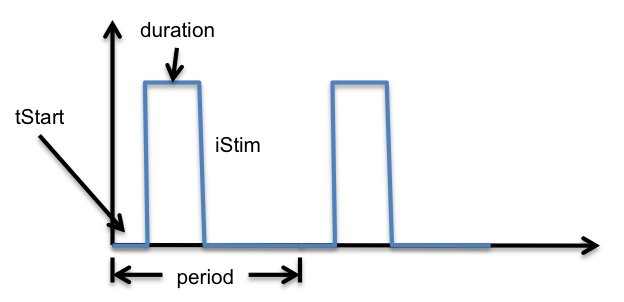
\includegraphics{graphics/pulseTrain.png}}
  \caption{Periodic pulse train.}
  \label{fig:pulseTrain}
\end{figure}

\issue{Jeremy has indicated that it is more natural to specify the
  stimulus current in units of current/volume rather than the stimulus
  voltage.  We will add an iStim keyword in a future version.}

\issue{The behavior of multiple STIMULUS objects is not carefully
  implemented.  Should it always be the sum?}

\issue{As implemented, the Stimulus class can access and modify the
  value of $dV/dt$ sue to diffusion.  This is a carry over from
  BlueBeats.  Is this a good idea?  Should we eliminate this possiblity?
   Should it be under keyword control?  Note that this imposes some
   potentially undesirable serialization constraints.}

\subsubsection{Box Stimulus}

Applies the stimulus to all cells inside a specified box.  \issue{The
  concept of inside a specified box is vague, especially since the cell
  can only be stimulated at a discretization point.  What about points
  that are on the boundary?  Should there be some kind of integration of
  the amount of volume associated with the point that is inside the box?
  This is closely related to the issue that the layout of the
  discretization in the box method for ANATOMY is not well defined.}

\begin{keywords}
  \kw{duration}{See Section~\ref{sssec:pulseTrains}.}{1~msec}
  \kw{period}{See Section~\ref{sssec:pulseTrains}.}{1000~msec}
  \kw{tStart}{See Section~\ref{sssec:pulseTrains}.}{1~msec}
  \kw{vStim}{See Section~\ref{sssec:pulseTrains}.}{-52~mV/msec}
  \kw{xMin}{Minimum grid index in the $x$-direction to stimulate.}{-1}
  \kw{xMax}{Maximum grid index in the $x$-direction to stimulate.}{Size of global grid in $x$-direction.}
  \kw{xMin}{Minimum grid index in the $y$-direction to stimulate.}{-1}
  \kw{xMax}{Maximum grid index in the $y$-direction to stimulate.}{Size of global grid in $y$-direction.}
  \kw{xMin}{Minimum grid index in the $z$-direction to stimulate.}{-1}
  \kw{xMax}{Maximum grid index in the $z$-direction to stimulate.}{Size of global grid in $z$-direction.}
\end{keywords}

\issue{Isn't it awkward that we specify the box in units of grid cells?
  Should it be in length units (like mm) instead?}


\subsubsection{Point Stimulus}
Applies the stimulus to a single cell specified by its global grid index.

\begin{keywords}
  \kw{cell}{The global grid index of the cell to stimulate.  See
    Section~\ref{sec:AnatomyFormat} for an explanation of the global grid
  index.}{0}
  \kw{duration}{See Section~\ref{sssec:pulseTrains}.}{1~msec}
  \kw{period}{See Section~\ref{sssec:pulseTrains}.}{1000~msec}
  \kw{tStart}{See Section~\ref{sssec:pulseTrains}.}{0~msec}
  \kw{vStim}{See Section~\ref{sssec:pulseTrains}.}{-52~mV/msec}
\end{keywords}

\subsubsection{Test Stimulus}
Intended for testing only.  Applies stimulus to a single cell specified
by a local index and an MPI rank.

\begin{keywords}
  \kw{cell}{The local index of the cell to stimulate.}{0}
  \kw{duration}{See Section~\ref{sssec:pulseTrains}.}{1~msec}
  \kw{period}{See Section~\ref{sssec:pulseTrains}.}{1000~msec}
  \kw{rank}{The MPI rank of the cell to stimulate.}{0}
  \kw{tStart}{See Section~\ref{sssec:pulseTrains}.}{1~msec}
  \kw{vStim}{See Section~\ref{sssec:pulseTrains}.}{-52~mV/msec}
\end{keywords}



\section{Anatomy File Format}
\label{sec:AnatomyFormat}

Anatom files are written using a parallel I/O system known as ``pio.''
The pio system is designed to provide extremely high I/O performance on
a variety of machines.  Because file-per-task and file-per-job
approaches to parallel I/O both have serious problems at large scale we
take a middle road and divide the data into $n$ physical files where $n$
is typically in the range of 1--2000.  For very large scale jobs and
highest throughput $n$ can be tuned according to the number of I/O nodes
on the system or some other hardware parameter that limits performance
such as the number of storage targets.


The filenames of the $n$ physical files in a pio logical file all share
common base name and end with the \#-sign and a six digit sequence
number.  For example, anatomy\#000000, anatomy\#000001, \ldots You can
think of this set of files as being logically concatenated in numerical
order.  Pio files may contain either ascii or binary data.

The zeroth file contains a human readable ascii header that describes
the data.  This header is of the form
\begin{verbatim}
name ClassName { 
  keyword1 = value1; 
  keyword2 = value2;
  ...
}
\end{verbatim}
Note that this is exactly the same form as an object in the object.data
input file.  Values may be string, floats, or integers and may be vector
or scalar valued.  Units are supported.  The set of keywords is open and
arbitrary.  You can put whatever data you want in the header to help
identify the file.  The maximum header length is something like 4k but
that could be easily extended if it became a limitation.  The header
ends with two newline characters in a row.

The header for an ascii anatomy file looks like this:
\begin{verbatim}
anatomy FILEHEADER{
  datatype = FIXRECORDASCII;
  nfiles = 1;
  nfields = 4;
  field_names = gid cellType theta phi;
  field_types = u u u u;
  nx = 3; ny = 3; nz = 3;
  nrecord = 27;
  lrec=12;
}
\end{verbatim}
The meaning of most of the keywords should be fairly self-evident.
\issue{However, this documentation should describe them and specify
  which keywords are manditory.}  Most are needed by pio to determine
how to read the file.  \issue{For now we're using ascii to facilitate
  debugging.  Binary files will be available in the future to improve
  performance and decrease storage cost.}


Note that the names and types of the data fields are specified.  

It is fairly simple to write reader code that is sensitive to the list
of data fields that are present.  For example the reader could notice
that only the cellType is in the file, read two columns instead of four
and synthesize the orientation data (or set a flag to tell someone else
it needs to be synthesized).

For ascii files the types can be f, u, and s, for integers, floats, and
strings.  Binary files have types such as i4, i8, f4, f8, b1, b2, b3, \ldots,
bn where bn is an unsigned integer stored in n bytes.

The gid field contains the 3D index of the cell converted to a single
integer by the formula $ix + nx*(iy + ny*iz)$.  (If necessary for
performance we could change this formula and use bit shifting operations
instead.)

The cell type field contains the cell type encoded according to the
following conventions:
\begin{center}
  \begin{tabular}{rl}
    75 & right ventricle endocardial cells\\
    76 & right ventricle m-cells\\
    77 & right ventricle epicardial cells\\
    100 & left ventricle endocardial cells\\
    101 & left ventricle m-cells\\
    102 & left ventricle epicardial cells\\
  \end{tabular}
\end{center}

The fibre angle is stored in theta and phi.  Theta is the polar angle,
phi the azimuthal.  In Blue Beats, angles were not stored as real
numbers in radians or degress, but rather as 8-bit unsigned integers.
We can choose to maintain this convention to save storage costs.  In
this convention the angle (in radians) is computed by the formula
$\theta\pi/256$ or $\varphi\pi/256$.  (In Blue Beats theta and phi were
effectively limited to values in the range [0..254]  This is not the
case in Cardioid.)

\issue{The coordinate system is not rigorously defined.  Presumeably
  theta is measured from the z-axis and phi from the x-axis.  This needs
  to be checked.  In any case I'm not familiar with the conventions of
  the field so I need some help here to make sure that we define things
  in a way that is consistent with conventions.}

All records (lines) must be exactly lrec long.  \issue{This is not quite
  true.  Fixed length records are a current implementation requirement,
  however, pio supports variable length records.  Somebody just needs to
  remember how to set up a reader that can use the variable record
  length features.}


\end{document}
%%% Local Variables: 
%%% mode: latex
%%% TeX-master: t
%%% End: 
